% ============================================================
% MATO-UAV Chapter 5 Figures - Usage Guide
% ============================================================
% Generated TikZ codes for 8 figures + comparison table
%
% PREAMBLE REQUIREMENTS:
% \usepackage{pgfplots}
% \pgfplotsset{compat=1.18}
% \usepackage{booktabs}
%
% USAGE IN YOUR DOCUMENT:
%
% Figure 1: Utility Convergence
% \begin{figure}[h]
% \centering
% 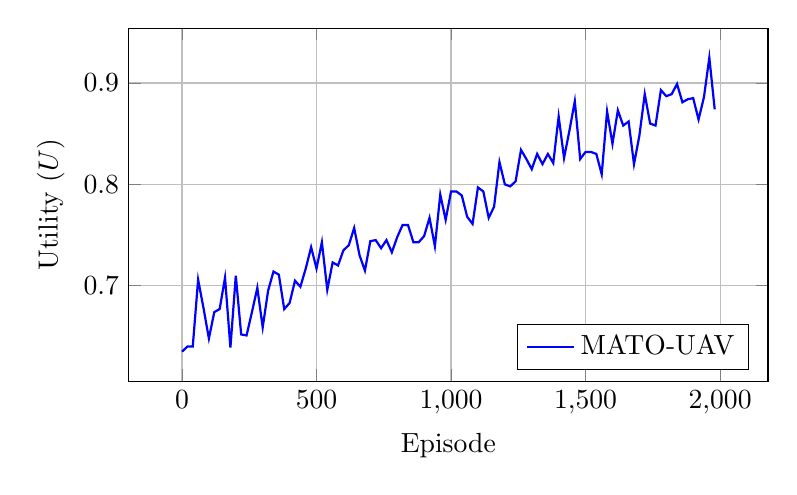
\begin{tikzpicture}
\begin{axis}[
    width=0.8\textwidth,
    height=0.5\textwidth,
    xlabel={Episode},
    ylabel={Utility ($U$)},
    grid=major,
    legend pos=south east
]
\addplot[blue, thick] coordinates {
(0,0.635) (20,0.640) (40,0.640) (60,0.706) (80,0.678) (100,0.648) (120,0.674) (140,0.677) (160,0.708) (180,0.639) (200,0.710) (220,0.652) (240,0.651) (260,0.674) (280,0.698) (300,0.659) (320,0.695) (340,0.714) (360,0.711) (380,0.677) (400,0.683) (420,0.705) (440,0.699) (460,0.717) (480,0.738) (500,0.717) (520,0.743) (540,0.696) (560,0.723) (580,0.720) (600,0.735) (620,0.740) (640,0.757) (660,0.730) (680,0.715) (700,0.744) (720,0.745) (740,0.737) (760,0.745) (780,0.733) (800,0.748) (820,0.760) (840,0.760) (860,0.743) (880,0.743) (900,0.749) (920,0.767) (940,0.739) (960,0.790) (980,0.765) (1000,0.793) (1020,0.793) (1040,0.789) (1060,0.768) (1080,0.761) (1100,0.797) (1120,0.793) (1140,0.767) (1160,0.778) (1180,0.822) (1200,0.800) (1220,0.798) (1240,0.803) (1260,0.834) (1280,0.825) (1300,0.815) (1320,0.830) (1340,0.820) (1360,0.830) (1380,0.821) (1400,0.867) (1420,0.826) (1440,0.853) (1460,0.882) (1480,0.825) (1500,0.832) (1520,0.832) (1540,0.830) (1560,0.810) (1580,0.872) (1600,0.840) (1620,0.873) (1640,0.858) (1660,0.862) (1680,0.820) (1700,0.848) (1720,0.889) (1740,0.860) (1760,0.858) (1780,0.893) (1800,0.887) (1820,0.889) (1840,0.899) (1860,0.881) (1880,0.884) (1900,0.885) (1920,0.864) (1940,0.886) (1960,0.925) (1980,0.874)
};
\legend{MATO-UAV}
\end{axis}
\end{tikzpicture}
% \caption{Utility convergence over training episodes}
% \label{fig:utility}
% \end{figure}
%
% Figure 2: Error Rate
% \begin{figure}[h]
% \centering
% 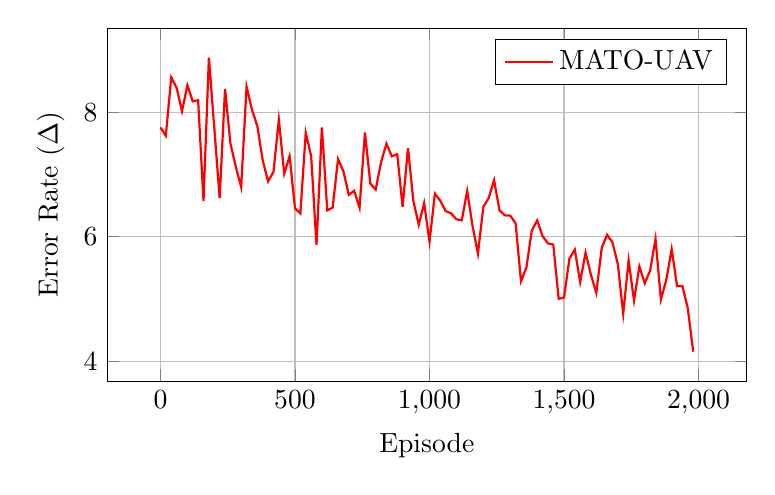
\begin{tikzpicture}
\begin{axis}[
    width=0.8\textwidth,
    height=0.5\textwidth,
    xlabel={Episode},
    ylabel={Error Rate ($\Delta$)},
    grid=major,
    legend pos=north east
]
\addplot[red, thick] coordinates {
(0,7.7537) (20,7.6217) (40,8.5574) (60,8.3913) (80,8.0138) (100,8.4304) (120,8.1736) (140,8.1916) (160,6.5762) (180,8.8751) (200,7.7512) (220,6.6195) (240,8.3739) (260,7.4974) (280,7.1255) (300,6.7980) (320,8.4100) (340,8.0401) (360,7.7775) (380,7.2281) (400,6.8869) (420,7.0396) (440,7.8785) (460,7.0131) (480,7.2925) (500,6.4566) (520,6.3735) (540,7.6688) (560,7.2981) (580,5.8685) (600,7.7549) (620,6.4247) (640,6.4676) (660,7.2461) (680,7.0524) (700,6.6728) (720,6.7376) (740,6.4638) (760,7.6742) (780,6.8531) (800,6.7583) (820,7.1990) (840,7.4948) (860,7.2897) (880,7.3254) (900,6.4809) (920,7.4228) (940,6.5732) (960,6.1908) (980,6.5401) (1000,5.9202) (1020,6.6900) (1040,6.5793) (1060,6.4116) (1080,6.3754) (1100,6.2789) (1120,6.2648) (1140,6.7338) (1160,6.1716) (1180,5.7310) (1200,6.4783) (1220,6.6217) (1240,6.9073) (1260,6.4246) (1280,6.3437) (1300,6.3389) (1320,6.2168) (1340,5.2864) (1360,5.5018) (1380,6.0958) (1400,6.2617) (1420,6.0122) (1440,5.8946) (1460,5.8743) (1480,5.0033) (1500,5.0253) (1520,5.6493) (1540,5.7941) (1560,5.2744) (1580,5.7457) (1600,5.3890) (1620,5.0997) (1640,5.8196) (1660,6.0315) (1680,5.9089) (1700,5.5590) (1720,4.7644) (1740,5.6213) (1760,4.9763) (1780,5.5243) (1800,5.2534) (1820,5.4581) (1840,5.9655) (1860,4.9935) (1880,5.3059) (1900,5.8023) (1920,5.2124) (1940,5.2051) (1960,4.8500) (1980,4.1552)
};
\legend{MATO-UAV}
\end{axis}
\end{tikzpicture}
% \caption{Error rate reduction during training}
% \label{fig:error}
% \end{figure}
%
% Figure 3: Stability
% \begin{figure}[h]
% \centering
% 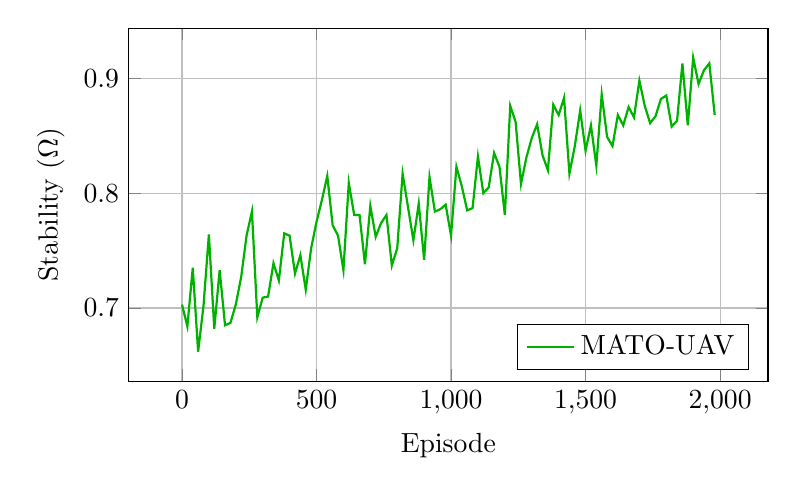
\begin{tikzpicture}
\begin{axis}[
    width=0.8\textwidth,
    height=0.5\textwidth,
    xlabel={Episode},
    ylabel={Stability ($\Omega$)},
    grid=major,
    legend pos=south east
]
\addplot[green!70!black, thick] coordinates {
(0,0.703) (20,0.684) (40,0.735) (60,0.662) (80,0.702) (100,0.764) (120,0.682) (140,0.733) (160,0.685) (180,0.687) (200,0.703) (220,0.727) (240,0.763) (260,0.784) (280,0.692) (300,0.709) (320,0.710) (340,0.739) (360,0.724) (380,0.765) (400,0.763) (420,0.730) (440,0.746) (460,0.716) (480,0.752) (500,0.775) (520,0.794) (540,0.815) (560,0.772) (580,0.763) (600,0.733) (620,0.809) (640,0.781) (660,0.781) (680,0.738) (700,0.789) (720,0.762) (740,0.774) (760,0.781) (780,0.737) (800,0.752) (820,0.817) (840,0.788) (860,0.759) (880,0.791) (900,0.742) (920,0.814) (940,0.784) (960,0.786) (980,0.790) (1000,0.763) (1020,0.823) (1040,0.806) (1060,0.785) (1080,0.787) (1100,0.832) (1120,0.800) (1140,0.805) (1160,0.835) (1180,0.823) (1200,0.781) (1220,0.876) (1240,0.862) (1260,0.808) (1280,0.831) (1300,0.848) (1320,0.860) (1340,0.833) (1360,0.820) (1380,0.877) (1400,0.868) (1420,0.883) (1440,0.817) (1460,0.841) (1480,0.872) (1500,0.837) (1520,0.859) (1540,0.824) (1560,0.886) (1580,0.849) (1600,0.841) (1620,0.868) (1640,0.859) (1660,0.875) (1680,0.866) (1700,0.898) (1720,0.876) (1740,0.861) (1760,0.867) (1780,0.882) (1800,0.885) (1820,0.858) (1840,0.863) (1860,0.913) (1880,0.859) (1900,0.918) (1920,0.895) (1940,0.907) (1960,0.913) (1980,0.868)
};
\legend{MATO-UAV}
\end{axis}
\end{tikzpicture}
% \caption{System stability improvement}
% \label{fig:stability}
% \end{figure}
%
% Figure 4: Pareto Front
% \begin{figure}[h]
% \centering
% % No valid Pareto points found
% \caption{Pareto-optimal solutions (Utility vs Error)}
% \label{fig:pareto}
% \end{figure}
%
% Figure 5: Energy Consumption
% \begin{figure}[h]
% \centering
% 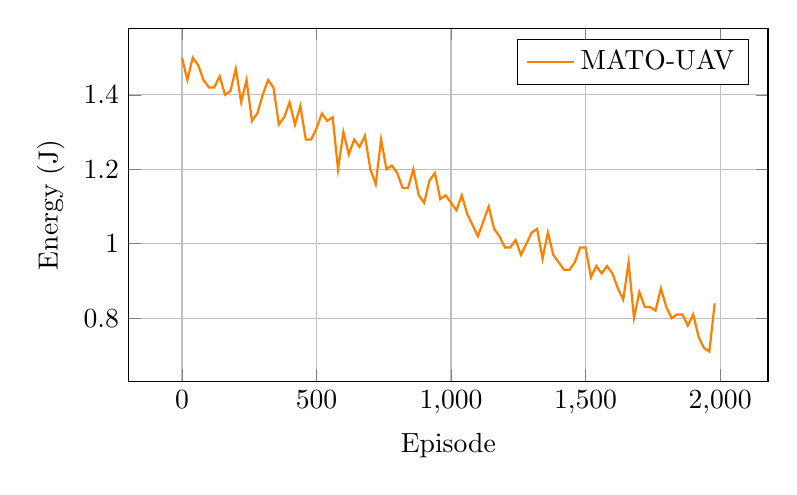
\begin{tikzpicture}
\begin{axis}[
    width=0.8\textwidth,
    height=0.5\textwidth,
    xlabel={Episode},
    ylabel={Energy (J)},
    grid=major,
    legend pos=north east
]
\addplot[orange, thick] coordinates {
(0,1.50) (20,1.44) (40,1.50) (60,1.48) (80,1.44) (100,1.42) (120,1.42) (140,1.45) (160,1.40) (180,1.41) (200,1.47) (220,1.38) (240,1.44) (260,1.33) (280,1.35) (300,1.40) (320,1.44) (340,1.42) (360,1.32) (380,1.34) (400,1.38) (420,1.32) (440,1.37) (460,1.28) (480,1.28) (500,1.31) (520,1.35) (540,1.33) (560,1.34) (580,1.20) (600,1.30) (620,1.24) (640,1.28) (660,1.26) (680,1.29) (700,1.20) (720,1.16) (740,1.28) (760,1.20) (780,1.21) (800,1.19) (820,1.15) (840,1.15) (860,1.20) (880,1.13) (900,1.11) (920,1.17) (940,1.19) (960,1.12) (980,1.13) (1000,1.11) (1020,1.09) (1040,1.13) (1060,1.08) (1080,1.05) (1100,1.02) (1120,1.06) (1140,1.10) (1160,1.04) (1180,1.02) (1200,0.99) (1220,0.99) (1240,1.01) (1260,0.97) (1280,1.00) (1300,1.03) (1320,1.04) (1340,0.96) (1360,1.03) (1380,0.97) (1400,0.95) (1420,0.93) (1440,0.93) (1460,0.95) (1480,0.99) (1500,0.99) (1520,0.91) (1540,0.94) (1560,0.92) (1580,0.94) (1600,0.92) (1620,0.88) (1640,0.85) (1660,0.95) (1680,0.80) (1700,0.87) (1720,0.83) (1740,0.83) (1760,0.82) (1780,0.88) (1800,0.83) (1820,0.80) (1840,0.81) (1860,0.81) (1880,0.78) (1900,0.81) (1920,0.75) (1940,0.72) (1960,0.71) (1980,0.84)
};
\legend{MATO-UAV}
\end{axis}
\end{tikzpicture}
% \caption{Energy consumption over episodes}
% \label{fig:energy}
% \end{figure}
%
% Figure 6: Delay Performance
% \begin{figure}[h]
% \centering
% 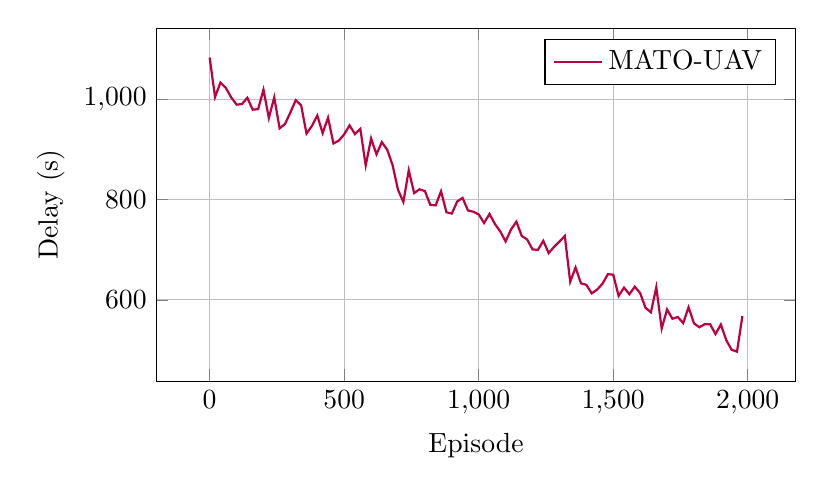
\begin{tikzpicture}
\begin{axis}[
    width=0.8\textwidth,
    height=0.5\textwidth,
    xlabel={Episode},
    ylabel={Delay (s)},
    grid=major,
    legend pos=north east
]
\addplot[purple, thick] coordinates {
(0,1083.333) (20,1004.753) (40,1033.333) (60,1023.079) (80,1003.817) (100,989.559) (120,990.680) (140,1003.260) (160,979.517) (180,980.556) (200,1019.347) (220,962.922) (240,1004.004) (260,942.191) (280,950.896) (300,974.020) (320,998.437) (340,988.109) (360,931.734) (380,947.029) (400,967.820) (420,932.679) (440,963.515) (460,912.072) (480,917.711) (500,930.375) (520,948.061) (540,930.800) (560,941.389) (580,868.101) (600,922.088) (620,890.386) (640,914.808) (660,899.345) (680,868.673) (700,819.577) (720,795.387) (740,858.455) (760,813.045) (780,820.585) (800,817.114) (820,789.656) (840,788.548) (860,816.702) (880,774.799) (900,772.172) (920,796.235) (940,803.476) (960,778.417) (980,775.924) (1000,770.603) (1020,753.423) (1040,771.424) (1060,751.632) (1080,736.654) (1100,716.692) (1120,740.283) (1140,755.989) (1160,727.467) (1180,720.592) (1200,700.751) (1220,699.783) (1240,717.746) (1260,693.492) (1280,705.706) (1300,716.266) (1320,727.571) (1340,636.148) (1360,664.603) (1380,633.067) (1400,630.002) (1420,613.001) (1440,620.463) (1460,632.240) (1480,651.242) (1500,650.214) (1520,607.922) (1540,624.466) (1560,611.231) (1580,626.335) (1600,613.564) (1620,584.121) (1640,575.247) (1660,625.202) (1680,542.734) (1700,580.904) (1720,562.314) (1740,565.819) (1760,553.576) (1780,585.278) (1800,553.280) (1820,545.332) (1840,551.521) (1860,551.395) (1880,531.878) (1900,550.735) (1920,519.838) (1940,500.440) (1960,496.663) (1980,567.733)
};
\legend{MATO-UAV}
\end{axis}
\end{tikzpicture}
% \caption{Delay performance improvement}
% \label{fig:delay}
% \end{figure}
%
% Figure 7: Energy-Delay Tradeoff
% \begin{figure}[h]
% \centering
% % No valid Energy-Delay points found
% \caption{Energy-Delay tradeoff analysis}
% \label{fig:energy_delay}
% \end{figure}
%
% Table: Comparison Table
% \begin{table}[h]
\centering
\caption{MATO-UAV Performance Summary}
\label{tab:mato_summary}
\begin{tabular}{lccr}
\toprule
\textbf{Metric} & \textbf{Initial} & \textbf{Final} & \textbf{Improvement} \\
\midrule
Utility ($U$)       & 0.635 & 0.886 & +39.5\% \\
Error Rate ($\Delta$) & 7.7537 & 4.9825 & -35.7\% \\
Stability ($\Omega$) & 0.703 & 0.855 & +21.7\% \\
Energy (J)          & 1.50 & 0.71 & -52.8\% \\
Delay (s)           & 1083.333 & 492.314 & -54.6\% \\
\bottomrule
\end{tabular}
\end{table}
%
% ============================================================